\begin{figure}[!ht]
    \centering
    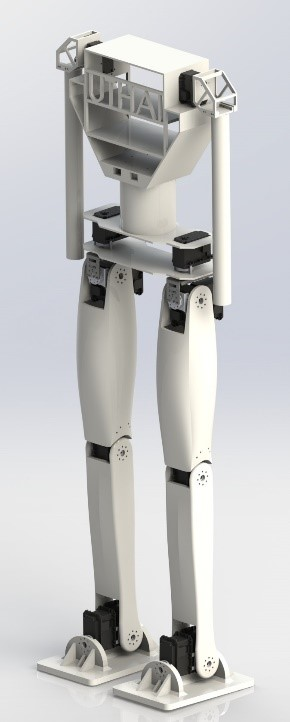
\includegraphics[width=0.2\textwidth]{chapter4/images/UTHAI_ver_1.jpg}
    \caption{โครงสร้างหุ่นยนต์ในโปรแกรม 3 มิติ}
    \label{fig:UTHAI_ver_1}
\end{figure}

โครงสร้างของหุ่นยนต์หลักๆจะแบ่งออกเป็น 2 ส่วนคือ ส่วนท่อนบนและส่วนท่อนล่างโดยส่วนท่อนบนจะประกอบไปด้วย 
เอว 1 ส่วน ลำตัว 1 ส่วน แขน 2 ส่วน และท่อนล่างจะประกอบไปด้วย สะโพก 1 ส่วน ขา 2 ส่วน น่อง 2 ส่วน ฝ่าเท้า 2 ส่วน 
ในการเลือกใช้วัสดุนั้นได้แสดงในตาราง 4.2

\begin{table}[ht]
	\centering
	\begin{tabular}{| l | l |}
		\hline
		ชิ้นส่วน & วัสดุที่ใช้ขึ้นรูป \\
        \hline
        แขน	& ท่อคาร์บอนไฟเบอร์ ขนาด 30 มม. \\
        ลำตัว & เครื่องพิมพ์ 3 มิติ โดยใช้วัสดุ PLA \\
        เอว	& ท่อคาร์บอนไฟเบอร์ ขนาด 88 มม. \\
        สะโพก & อลูมิเนียมอัลลอยพับ \\
        น่อง & เครื่องพิมพ์ 3 มิติ โดยใช้วัสดุ PLA \\
        ขา & เครื่องพิมพ์ 3 มิติ โดยใช้วัสดุ PLA \\
        ฝ่าเท้า	& เครื่องพิมพ์ 3 มิติ โดยใช้วัสดุ PLA \\
	    \hline
	\end{tabular}
	\caption{ตารางแสดงวัสดุที่ใช้ขึ้นรูป UTHAI}
	\label{tab:UTHAI_material}
\end{table}

\clearpage
\subsection{การออกแบบขา}
\subsubsection{การออกแบบโครงสร้างส่วนขาครั้งที่ 1}
การออกแบบโครงสร้างส่วนขาของหุ่นยนต์ฮิวมานอยด์ ได้ออกแบบโดยคำนึงถึงการขึ้นรูปด้วยเครื่องพิมพ์สามมิติ (3D Printer) 
แต่เนื่องจากว่าเครื่องพิมพ์สามมิติที่ใช้ในการผลิตนั้นมีขนาดที่เล็กกว่าขนาดที่จะพิมพ์จริงจึงต้องทำการแยกส่วนของขาออก
เป็นจำนวน 2 ส่วนในแต่ละในก้านต่อของขาท่อนบนและขาท่อนล่าง และหลังจากนั้นใช้การยึดชิ้นส่วนด้วยการตอกสลักเพื่อยึดติดชิ้นส่วนเข้าด้วยกัน
เพื่อให้มีความแข็งแรงมากกว่าการต่อแบบทั่วไป

\begin{figure}[!ht]
    \centering
    \begin{subfigure}[b]{0.3\linewidth}
      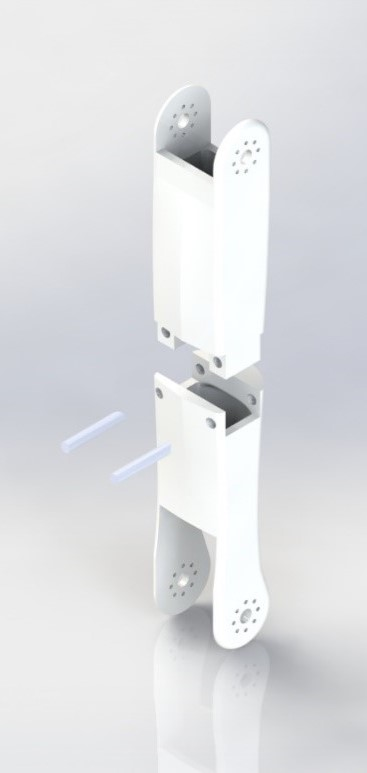
\includegraphics[width=\linewidth]{chapter4/images/shin.jpg}
      \caption{โครงสร้างส่วนหน้าแข้ง}
    \end{subfigure}
    \begin{subfigure}[b]{0.35\linewidth}
      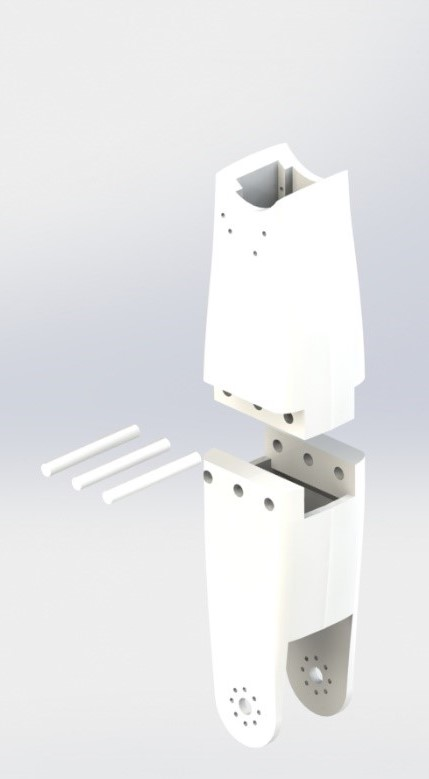
\includegraphics[width=\linewidth]{chapter4/images/thigh.jpg}
      \caption{โครงสร้างส่วนต้นขา}
    \end{subfigure}
    \caption{รูปการออกแบบส่วนขาของหุ่นยนต์อุทัย}
    \label{fig:leg}
  \end{figure}

เมื่อทำการพิมพ์ชิ้นงานส่วนขาท่อนบนและท่อนล่าง ออกมาจะได้น้ำหนักของชิ้นงานตามตาราง \ref{tab:UTHAI_leg}
\begin{table}[ht]
	\centering
	\begin{tabular}{| l | l |}
		\hline
		ชิ้นส่วน & น้ำหนัก(กรัม) \\
        \hline
        ต้นขา & 263 \\
        หน้าแข้ง & 204 \\
	    \hline
	\end{tabular}
	\caption{ตารางแสดงน้ำหนักของชิ้นส่วนขา}
	\label{tab:UTHAI_leg}
\end{table}

จากการทดสอบความสามารถในการเคลื่อนที่ พบว่าตัวขับเคลื่อนสามารถเคลื่อนที่เข้าตำแหน่งได้ถูกต้องตามมุม 
ที่ป้อนเข้าไปให้ระบบ แต่หากทำให้ชิ้นส่วนของขาเคลื่อนที่ด้วยถี่ไปกลับสูงและด้วยความเร็วที่มาก จะทำให้ตัวขับเคลื่อนเกิดการโอเวอร์โหลด 
ซึ่งมีผลทำตัวขับเคลื่อนหยุดการทำงาน ซึ่งต้องทำการปิดเปิดตัวขับเคลื่อนใหม่

\clearpage
\subsubsection*{ผลการทดสอบ}
จากการทดสอบความแข็งแรงของชิ้นงาน พบว่าชิ้นงานมีความแข็งแรงเพียงพอที่จะทำให้ตัวขับเคลื่อนมีค่าแรงบิดเป็นค่าแรงบิดสูงสุด(Stall Torque)
แล้วทำให้ชิ้นงานไม่เกิดความเสียหาย

จากการทดสอบระยะเวลาการทำงานของตัวขับเคลื่อน ด้วยการเขียนโปรแกรมให้ตัวขับเคลื่อน เคลื่อนที่ไปกลับ สลับตำแหน่งไปเรื่อยๆอย่างต่อเนื่อง เป็นเวลา 20 นาที
พบว่า ตัวขับเคลื่อนทำงานได้เป็นปกติ

\subsubsection*{ปัญหาที่พบในการออกแบบครั้งที่ 1}
เนื่องจากว่าเป้าหมายของการสร้างหุ่นยนต์ตัวนี้ให้มีน้ำหนักที่เบา (น้อยกว่า 5 กิโลกรัม) จึงพบปัญหาว่า
น้ำหนักของส่วนขาที่ได้ออกแบบมานั้นมีน้ำหนักมากเกินกว่าของหุ่นยนต์กนก(ชื่อหุ่นยนต์ตัวเดิมก่อนจะเป็นอุทัย)
ซึ่งเป็นผลทำให้เกิดปํญหาเรื่องภาระโหลดของ motor ที่ต้องกระทำที่มีมากขึ้นจากเดิมและจะทำให้น้ำหนักของตัวหุ่นยนต์มากขึ้น 
เมื่อเปรียบเทียบผลลัพธ์น้ำหนักส่วนขาของหุ่นยนต์กนกกับหุ่นยนต์อุทัยแล้วได้ผลดังตาราง \ref{tab:UTHAI_KANOK_Comp}

\begin{table}[ht]
	\centering
	\begin{tabular}{| l | l | l |}
		\hline
        ชิ้นส่วน & หุ่นยนต์กนก(เดิม)(กรัม) & หุ่นยนต์ UTHAI \\
        \hline
        ขาท่อนบน & 171 & 263 \\
        ขาท่อนล่าง & 172 & 204 \\
	    \hline
	\end{tabular}
	\caption{ตารางเปรียบเทียบน้ำหนักของชิ้นส่วนขาของหุ่นยนต์}
	\label{tab:UTHAI_KANOK_Comp}
\end{table}

จากข้อมูลในตารางนั้นจะเห็นได้ว่า หนักที่เพิ่มขึ้นมากจากการออกแบบใหม่แต่ละชิ้นนั้น มากถึง 124 กรัม
ต่อขา 1 ข้าง และ 248 กรัมเมื่อเทียบกับขาทั้งหมดและเปรียบเทียบกับข้อมูลก่อนหน้า

หลังจากพบปัญหาดังกล่าวผู้จัดทำจึงได้ตัดสินใจทำการเปลี่ยนวัสดุที่ใช้ทำโครงสร้างในครั้งแรก
ที่จะใช้การขึ้นรูปชิ้นงานด้วยการพิมพ์ขึ้นรูป 3 มิติ มาเป็นวัสดุผลระหว่างคาร์บอนไฟเบอร์และชิ้นงาน 3 มิติแทน
โดยจะให้ชิ้นงาน 3 มิตินั้นทำหน้าที่เป็นตัวเชื่อมระหว่างวัสดุคาร์บอนไฟเบอร์กับมอเตอร์ และยึดกับวัสดุคาร์บอนไฟเบอร์ด้วยการบีบ
ซึ่งเหตุผลที่ต้องทำเช่นนี้เพราะต้องการลดน้ำหนักของหุ่นยนต์ลง เพื่อไม่ให้มอเตอร์รับภาระที่หนักเกินไป 

\begin{table}[ht]
	\centering
	\begin{tabular}{| l | l | l |}
		\hline
		ชิ้นส่วน & วัสดุที่ใช้ขึ้นรูป(เก่า) & วัสดุที่ใช้ขึ้นรูป(ใหม่) \\
        \hline
        แขน	& ท่อคาร์บอนไฟเบอร์ ขนาด 30 มม. & เดิม\\
        ลำตัว & เครื่องพิมพ์ 3 มิติ โดยใช้วัสดุ PLA & เดิม\\
        เอว	& ท่อคาร์บอนไฟเบอร์ ขนาด 88 มม. & เดิม\\
        สะโพก & อลูมิเนียมอัลลอยพับ & เดิม\\
        น่อง & เครื่องพิมพ์ 3 มิติ โดยใช้วัสดุ PLA & วัสดุผสมระหว่างคาร์บอนไฟเบอร์และ ชิ้นงาน 3 มิติ \\
        ขา & เครื่องพิมพ์ 3 มิติ โดยใช้วัสดุ PLA  & วัสดุผสมระหว่างคาร์บอนไฟเบอร์และ ชิ้นงาน 3 มิติ\\
        ฝ่าเท้า	& เครื่องพิมพ์ 3 มิติ โดยใช้วัสดุ PLA & เดิม\\
	    \hline
	\end{tabular}
	\caption{ตารางแสดงวัสดุที่แก้ไขในการใช้ขึ้นรูป UTHAI }
	\label{tab:UTHAI_materialchange}
\end{table}

\clearpage
\subsubsection{การออกแบบโครงสร้างส่วนขาครั้งที่ 2}
ครั้งนี้การออกแบบชิ้นส่วนขาของหุ่นยนต์นั้น ได้คำนึงถึงเรื่องน้ำหนักเป็นหลัก และยังคงให้ความสำคัญกับข้อต่อที่จะใช้รับน้ำหนักทั้งตัวหุ่นยนต์
และยังคงรับแรงบิดของมอเตอร์อีกด้วย ดังนั้นจึงได้ตัดสินใจที่จะเปลี่ยนจากการใช้วัสดุ 3D print  ซึ่งเป็นพลาสติกทั้งหมด มาเป็นวัสดุผสม 
ระหว่าง Carbonfiber กับ 3D print ซึ่งขึ้นรูปจากพลาสติก PLA และทำการยึดติดกันด้วยการบีบอัดดังรูปที่\ref{fig:newleg}
เมื่อทำการพิมพ์ชิ้นงานส่วนขาท่อนบนและท่อนล่างและทำการประกอบ จะได้น้ำหนักของชิ้นงานเปรียบเทียบกับของเดิมดังตามตาราง\ref{tab:UTHAI_leg_compilation}

\begin{figure}[!ht]
    \centering
    \begin{subfigure}[b]{0.3\linewidth}
      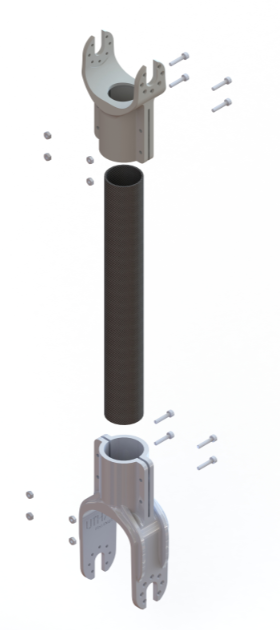
\includegraphics[width=\linewidth]{chapter4/images/carb_shin.PNG}
      \caption{โครงสร้างส่วนหน้าแข้ง (ใหม่)}
    \end{subfigure}
    \begin{subfigure}[b]{0.3\linewidth}
      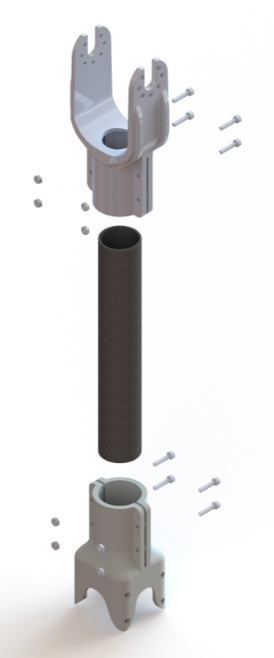
\includegraphics[width=\linewidth]{chapter4/images/carb_thigh.PNG}
      \caption{โครงสร้างส่วนต้นขา (ใหม่)}
    \end{subfigure}
    \caption{รูปการออกแบบส่วนขาของหุ่นยนต์อุทัย (ใหม่)}
    \label{fig:newleg}
  \end{figure}

\begin{table}[!ht]
	\centering
	\begin{tabular}{| l | l | l |}
		\hline
		ชิ้นส่วน & น้ำหนักเดิม(กรัม) & น้ำหนักใหม่(กรัม) \\
        \hline
        ต้นขา & 263 & 161\\
        หน้าแข้ง & 204 & 166\\
	    \hline
	\end{tabular}
	\caption{ตารางแสดงน้ำหนักเปรียบเทียบของชิ้นส่วนขา}
	\label{tab:UTHAI_leg_compilation}
\end{table}  

\clearpage
\subsubsection*{การขึ้นรูปชิ้นงาน}
การขึ้นรูปชิ้นงานนนั้น ได้ใช้การขึ้นรูปชิ้นตามความสูงแนวแกน Z ดังภาพ \ref{fig:print_axis} เพื่อให้ชิ้นงานมีความสวยงามและสามารถสวมได้พอดี
กับท่อนคาร์บอนโดยให้มีผิวสัมผัสมากที่สุด ในการยึดเกาะ\footnote{Experimental Characterization of the Mechanical Properties of 3D-Printed ABS and Polycarbonate Parts}
\begin{figure}[!ht]
    \centering
    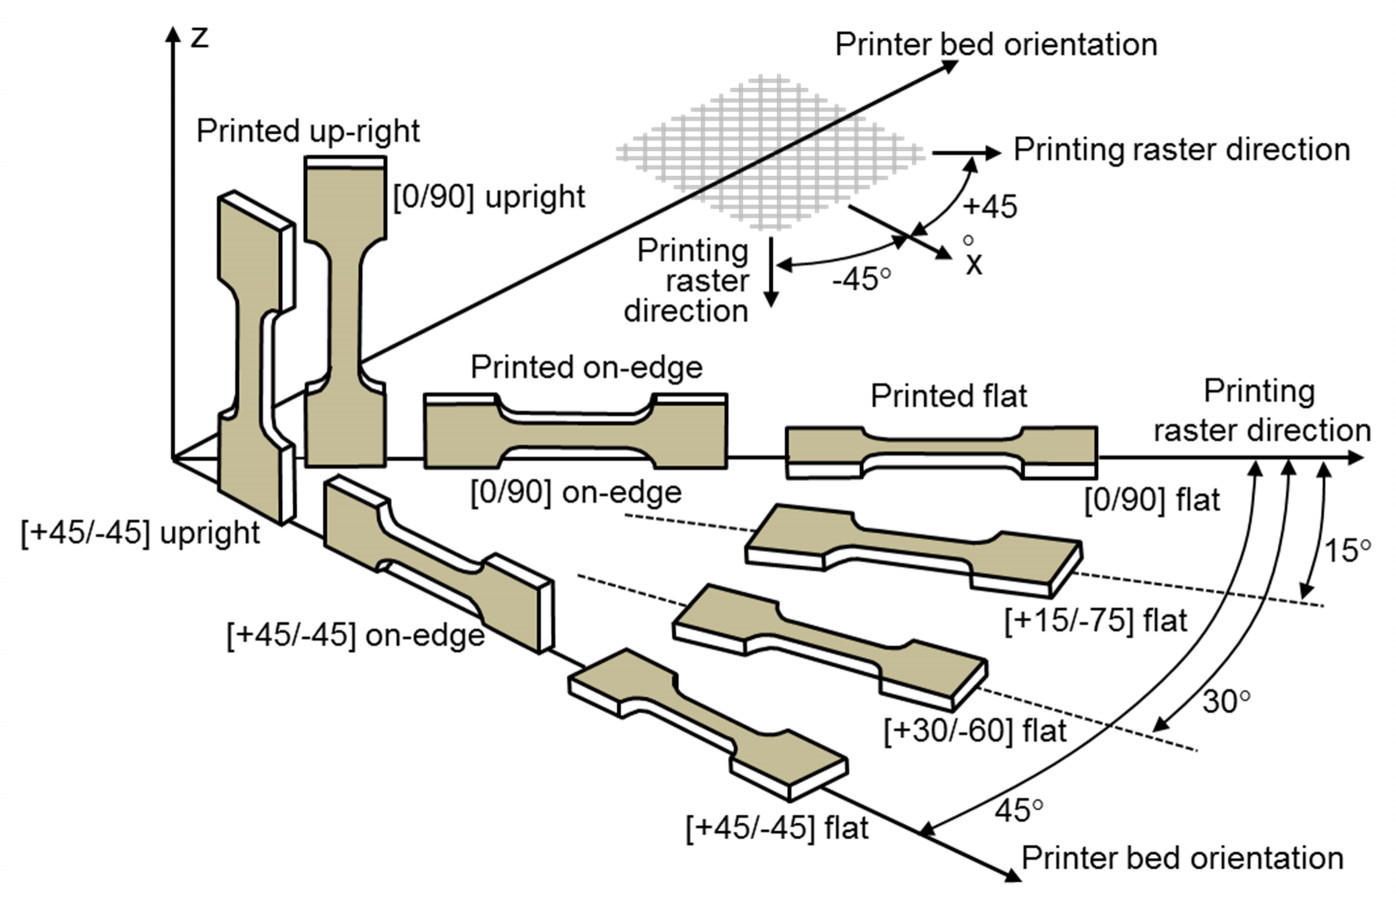
\includegraphics[width=0.6\textwidth]{chapter4/images/print_axis.png}
    \caption{รูปการชิ้นรูปชิ้นงานของ 3D printer }
    \label{fig:print_axis}
\end{figure}

\subsubsection{ทดสอบโครงสร้างและการขับเคลื่อน}	
จากการทดสอบความแข็งแรงของวัสดุโดยการนำไปประกอบกับตัวหุ่นยนต์จริง และทำการทดลองเดินพบว่าเมื่อทำการเดินจริงนั้น 
เกิดการฉีกขาดของชิ้นงานที่ ชั้นการพิมพ์ของชิ้นงานดังภาพ 4.9 ซึ่งเกิดจากการได้รับแรงบิดมากเกินไปจากน้ำหนักของชิ้นงานส่วนขา
และแรงที่ชิ้นงานจะได้รับนั้น จะเป็นเพียงส่วนการเชื่อมกันติดของชั้นพลาสติกเท่านั้น ซึ่ง ณ ที่นี้เส้นพลาสติกจะไม่ได้เป็นตัวรับแรงจึงทำให้
เกิดการเปราะหักที่ง่ายกว่าดังนั้นจึงทำการออกแบบใหม่โดยการเพิ่มสันให้ชิ้นงานและเพื่มความหนาบนหน้าแปลนเชื่อมกับตัวมอเตอร์
และทำการขึ้นรูปชิ้นงาน โดยให้ความสูงของชิ้นงานเป็นไปตามแกน X และทำการเติมเนื้อพลาสติกด้านในให้เต็ม 100\% ดังรูปที่ \ref{fig:fatiguelayer}
\begin{figure}[!ht]
    \centering
    \begin{subfigure}[b]{0.2\linewidth}
      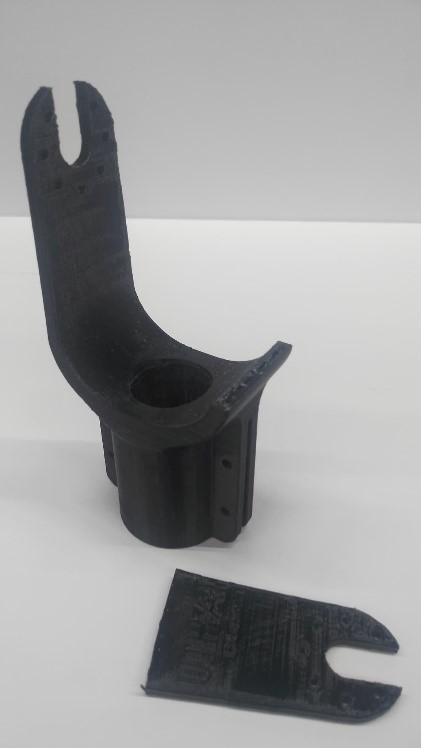
\includegraphics[width=\linewidth]{chapter4/images/fatigue1.jpg}
      \caption{รูปแสดงการแตกหักของชิ้นงาน}
    \end{subfigure}
    \begin{subfigure}[b]{0.3\linewidth}
      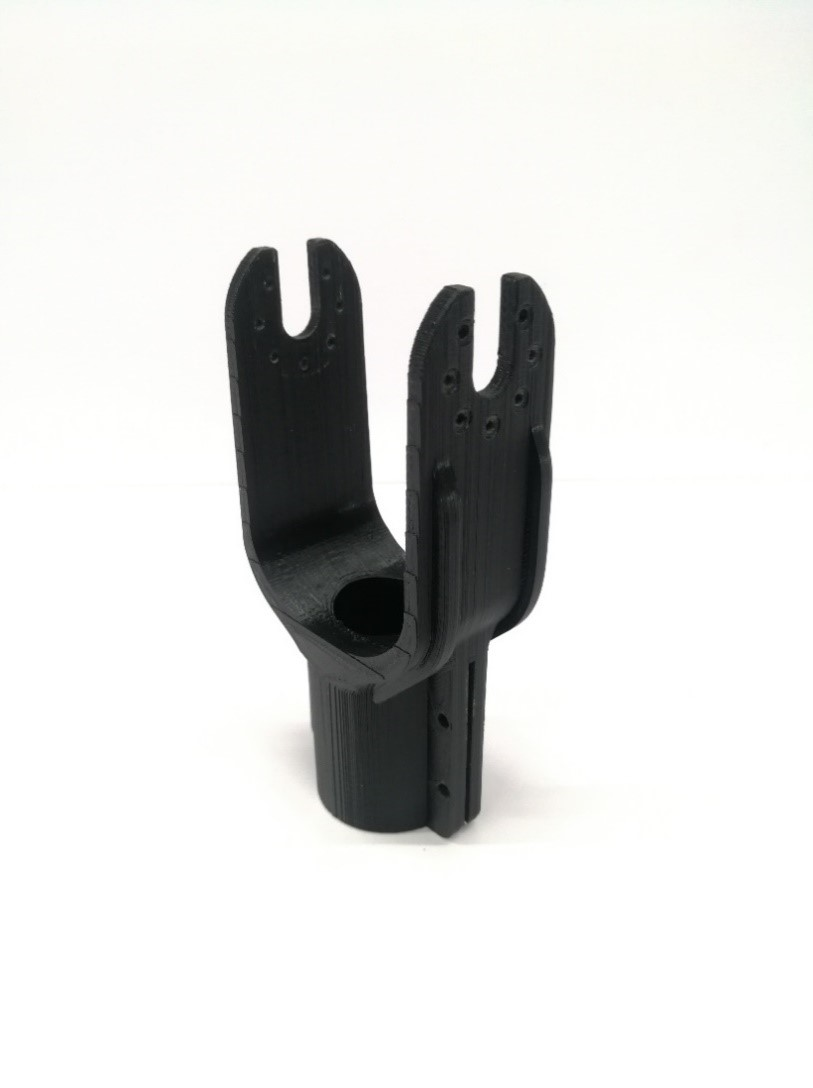
\includegraphics[width=\linewidth]{chapter4/images/fatigue2.jpg}
      \caption{รูปแสดงชิ้นงานที่ทำการออกแบบใหม่}
    \end{subfigure}
    \begin{subfigure}[b]{0.4\linewidth}
        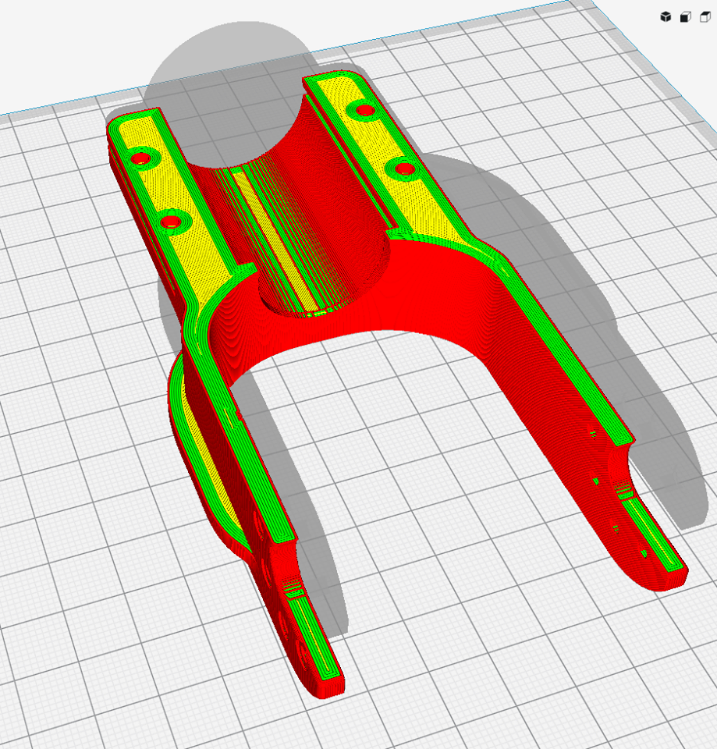
\includegraphics[width=\linewidth]{chapter4/images/fatigue3.png}
        \caption{รูปแสดงชั้นของการพิมพ์ตามแนวแกน x โดยการเติมเนื่อพลาสติก 100\%}
    \end{subfigure}
    \caption{รูปแสดงการแตกหักและชั้นการพิมพ์}
    \label{fig:fatiguelayer}
  \end{figure}

\subsubsection*{การทดลองความแข็งแรงของชิ้นงานโดยวิธีการวิเคราะห์เชิงตัวเลข(Finite element)}
ก่อนที่จะนำชิ้นงานที่ทำการออกแบบใหม่ที่เติมเนื่อพลาสติก 100\% ไปใช้งานจริงนั้นจะต้องผ่านการวิเคราะห์แรงกระทำ
โดยผ่านโปรแกรมจำลองเพื่อหาจุดที่เปราะบางของชิ้นงาน  และนำข้อมูลนั้นไปวิเคราะห์เพื่อปรับปรุงชิ้นงานต่อไป 
ซึ่งได้ตั้งค่า คุณสมบัติของชิ้นงาน 3d print ไว้ดังนี้ 
\begin{table}[ht]
	\centering
	\begin{tabular}{| l | l |}
		\hline
		Print Orientation Side	& flat \\
        \hline
        Ultimate Stress$(N/mm²)$\footnote{Tensile Testing of 3D Printed Materials for Scoliosis Brace( Rahul Malik)} & 	45.66 \\
        Young’s Modulus$(N/mm²)$\footnote{Tensile Testing of 3D Printed Materials for Scoliosis Brace( Rahul Malik)} & 	1141.55 \\
        Yield strength$(N/mm²)$\footnote{What is the influence of infill \%, layer height and infill pattern on my 3D prints (3D Matter)} & 23 \\
        Density$(kg/m^3)$\footnote{Filament volume and length(toybuilderlabs)} &	1250 \\
        Passion ratio\footnote{Additive Manufacturing and Characterization of Polylactic Acid (PLA) Composites ContainingMetal Reinforcements(NASA)} &	0.33 \\
        Force(torque)$(N.m)$ & 10.4 \\
	    \hline
	\end{tabular}
	\caption{ตารางแสดงค่าคุณสมบัติของวัสดุ 3D print(PLA)}
	\label{tab:PLA_property}
\end{table}

เมื่อทดลองนำค่าดังกล่าวไปใช้ในโปรแกรม solidwork และใช้ฟังก์ชัน mass property(คุณสมบัติของวัสดุ) เพื่อหาค่าน้ำหนักที่ผ่านการคำนวณโดยโปรแกรม
และนำมาเทียบกับชิ้นงานจริงเพื่อดูว่ามีความคลาดเคลื่อนด้านน้ำหนักมากน้อยขนาดไหน พบว่าค่าข้อมูลความคลาดเคลื่อนนั้นจะไม่เกินกว่าระหว่าง $\pm 1\%$ กับค่าที่แสดงบนโปรแกรม
หลังจากนั้นทำการวิเคราะห์ผ่านโปรแกรม solidword ด้วยการวิเคราะห์ FEA ได้ผลลัพธ์ ดังนี้

\begin{figure}[!ht]
  \centering
  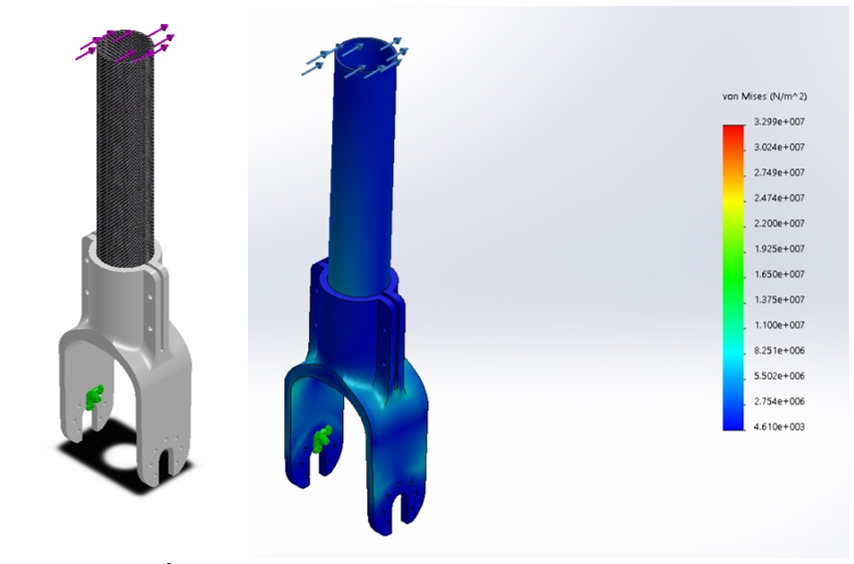
\includegraphics[width=0.8\textwidth]{chapter4/images/FEA1.PNG}
  \caption{รูปการวิเคราะห์แรงของข้อต่อ 1}
  \label{fig:FEAjoint1}
\end{figure}

\clearpage
\begin{figure}[!ht]
  \centering
  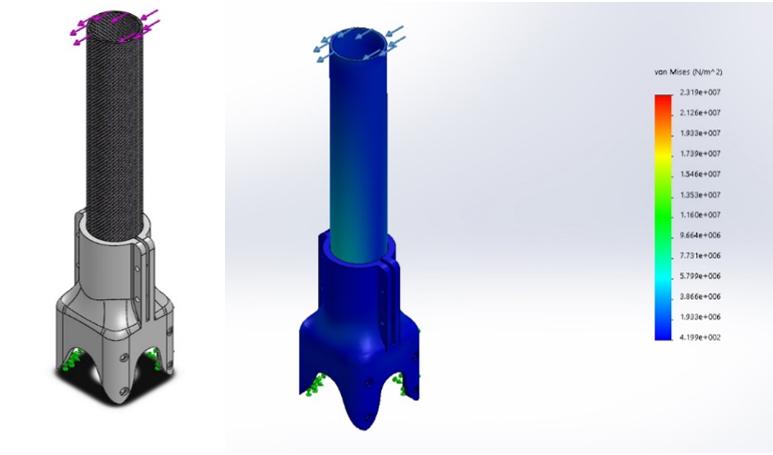
\includegraphics[width=0.8\textwidth]{chapter4/images/FEA2.PNG}
  \caption{รูปการวิเคราะห์แรงของข้อต่อ 2}
  \label{fig:FEAjoint2}
\end{figure}

\begin{figure}[!ht]
  \centering
  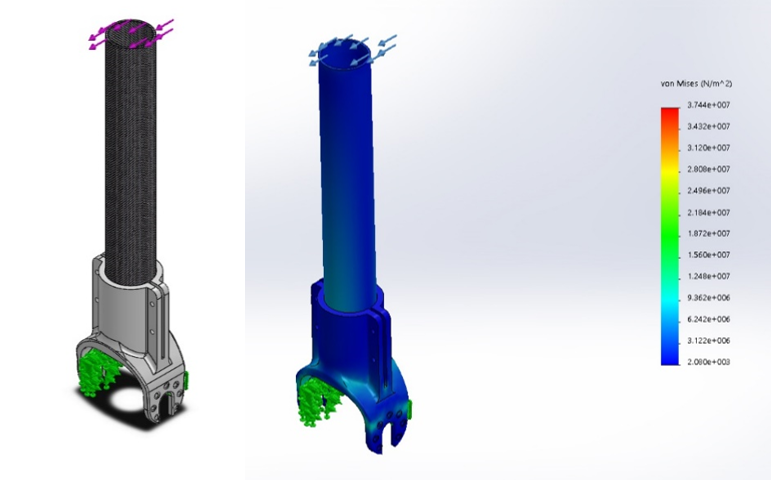
\includegraphics[width=0.8\textwidth]{chapter4/images/FEA3.PNG}
  \caption{รูปการวิเคราะห์แรงของข้อต่อ 3}
  \label{fig:FEAjoint3}
\end{figure}
\clearpage

การวิเคราะห์นั้นจะทำการยึดจุดที่เป็นหน้าแปลนของมอเตอร์ไว้เพื่อให้เปรียบเสมือนกับว่าขณะนี้ชิ้นงาน
ได้เชื่อมติดกับตัวมอเตอร์ หลังจากนั้นกำหนดแรงกระทำเพื่อให้เกิดโมเมนต์กับชิ้นงานโดยค่าแรงที่กระทำนั้น
ได้มาจากการคำณวนแรงของมอเตอร์ที่จะรับไหวเทียบกับระยะของแรง ที่กระทำกับชิ้นงาน 
ซึ่งได้ทดลองกับชิ้นงานตัวข้อต่อ 1 2 และ 3 ด้วยแรง 41.6 นิวตัน$(N)$
เมื่อนำค่า ความตึงเครียดสูงสุด$(Max stress)$ของชิ้นงานมาวิเคราะห์เพื่อหา จุดเปราะบางของวัสดุได้ค่าดังตาราง
\ref{tab:streaa_result}
\begin{table}[ht]
	\centering
	\begin{tabular}{| l | c |}
		\hline
		ชื่อชิ้นงาน	& ความตึงเครียดสูงสุดของชิ้นงาน(Max stress)$(N/mm^2)$ \\
        \hline
        ข้อต่อ 1 & 32.99 \\
        ข้อต่อ 2 & 23.19 \\
        ข้อต่อ 3 & 7.987 \\
	    \hline
	\end{tabular}
	\caption{ตารางแสดงความตึงเครียดของชิ้นงาน(Stress)}
	\label{tab:stress_result}
\end{table}

จากผลการทดลองสรุปได้ว่า ค่าความตึงเครียดต่างๆที่ได้มาจากผลลัพธ์นั้นเมื่อนำไปเทียบกับค่าความตึงเครียดสูงสุดที่วัสดุจะรับไหว
ที่ 45.66 N/mm² เห็นได้ว่ายังคงไม่มีวัสดุตัวไหนที่จะเกิดการแตกหักเมื่อเกิดแรงกระทำกับชิ้นงานดังนั้นชิ้นงานที่ทำการออกแบบนี้
พอสรุปได้ว่าจะไม่เกิดการแตกหักระหว่างการทำงาน ยกแว้นมีแรงกระทำจากภายนอกที่มากเกินไปจนมาผลทำให้เกิดความตึงเครียดของชิ้นงานสูง
เกินกว่าค่าดังกล่าว  

\clearpage
\subsection{การออกแบบเท้า}
\subsubsection{การออกแบบโครงสร้างเท้าครั้งที่ 1}
โครงสร้างเท้านั้นได้ออกแบบให้มีลักษณะคล้ายคลึงกับรองเท้าของมนุษย์จริงและมีขนาดที่เหมาะสมกับตัวหุ่นยนต์ โดยคำนึงถึงความแข็งแรง
และการใช้งานเป็นหลัก และยังต้องขึ้นรูปด้วยเครื่องพิมพ์ 3 มิติได้อีกด้วย
\begin{figure}[h!]
  \centering
  \begin{subfigure}[b]{0.55\linewidth}
    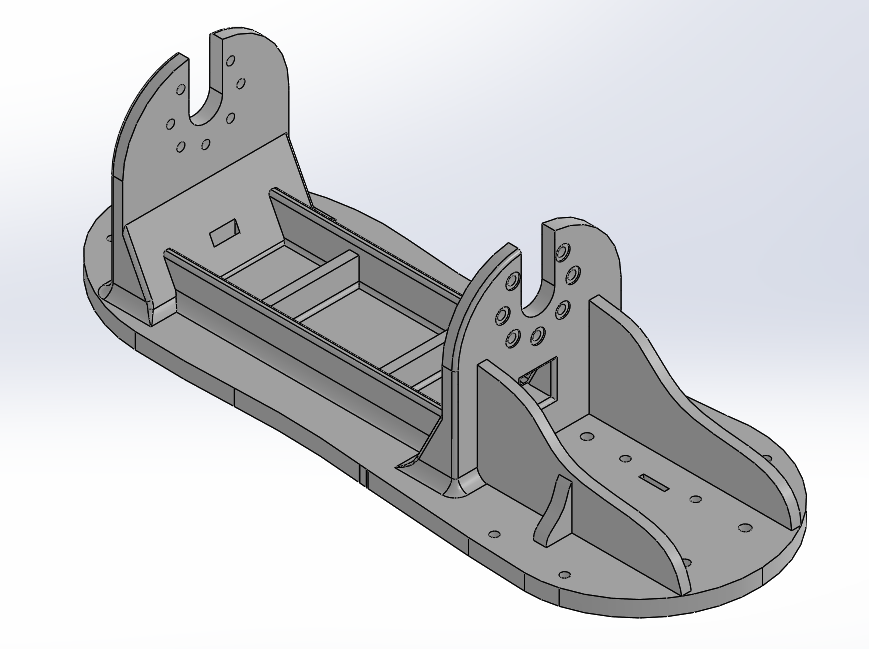
\includegraphics[width=\linewidth]{chapter4/images/foot_old.PNG}
    \caption{รูปแสดงเท้าของหุ่นยนต์}
  \end{subfigure}
  \begin{subfigure}[b]{0.2\linewidth}
    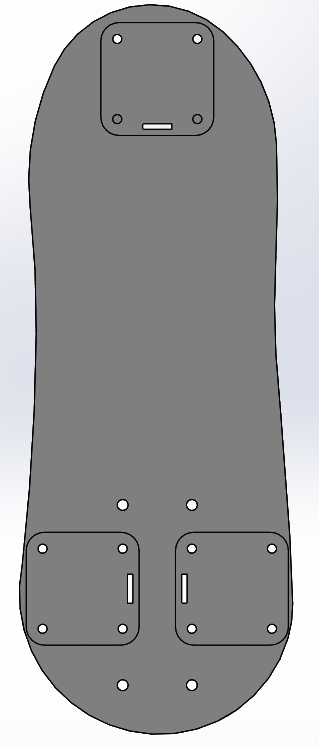
\includegraphics[width=\linewidth]{chapter4/images/bare_footold.PNG}
    \caption{รูปแสดงฝ่าเท้าของหุ่นยนต์}
  \end{subfigure}
  \caption{รูปแสดงเท้าของหุ่นยนต์อุทัย}
  \label{fig:footold}
\end{figure}

\clearpage
ในส่วนของโครงครอบ FSR นั้นได้ออกแบบให้มีการกดโดยตรงกับหน้าสัมผัสซึ่งส่วนที่สัมผัสกับหน้าสัมผัสนั้นจะเป็นเฉพาะส่วนของ 3d print ที่ออกแบบมา
เฉพาะการกดโดยเฉพาะ ซึ่งจะทำให้ถนอมหน้าสัมผัสได้ดีกว่า การกดจากภายนอกโดยตรงซึ่งตัวเซนเซอร์นี้จะมีความสูงออกมาจากฝ่าเท่าเป็นระยะ 5.4 มิลลิเมตร 
โดยจะมีจำนวน 3 ตัวต่อเท้า 1 ข้าง
\begin{figure}[!ht]
  \centering
  \begin{subfigure}[b]{0.4\linewidth}
    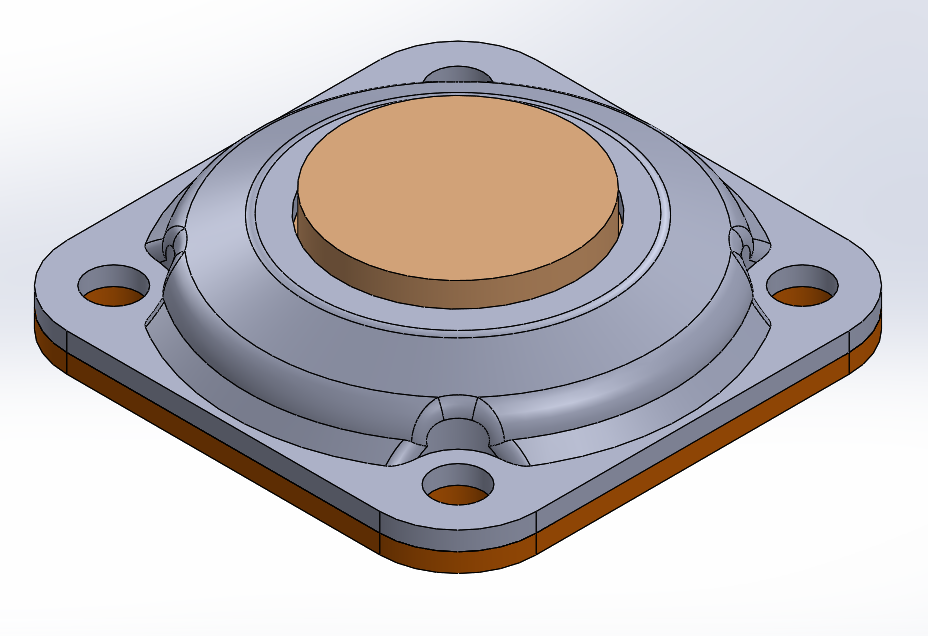
\includegraphics[width=\linewidth]{chapter4/images/FSR.PNG}
    \caption{รูปแสดงโครงครอบ FSR}
  \end{subfigure}
  \begin{subfigure}[b]{0.5\linewidth}
    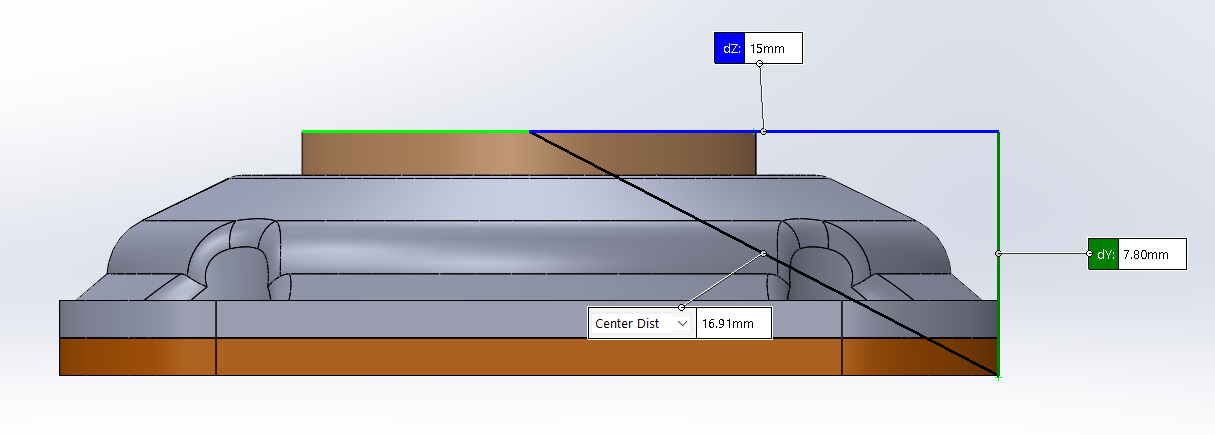
\includegraphics[width=\linewidth]{chapter4/images/FSR_mensure.PNG}
    \caption{รูปแสดงขนาดโครงครอบ FSR}
  \end{subfigure}
  \caption{รูปแสดงโดยรวมของโครงครอบ FSR}
  \label{fig:FSR}
\end{figure}

\subsubsection*{การทดลองความแข็งแรงของชิ้นงานโดยวิธีการวิเคราะห์เชิงตัวเลข(Finite element)}
จากค่าคุณสมบัติของชิ้นงานดังตาราง \ref{tab:PLA_property} นำมาวิเคราะห์ด้วยเทคนิคเชิงตัวเลขได้ผลดังนี้
\begin{figure}[!ht]
  \centering
  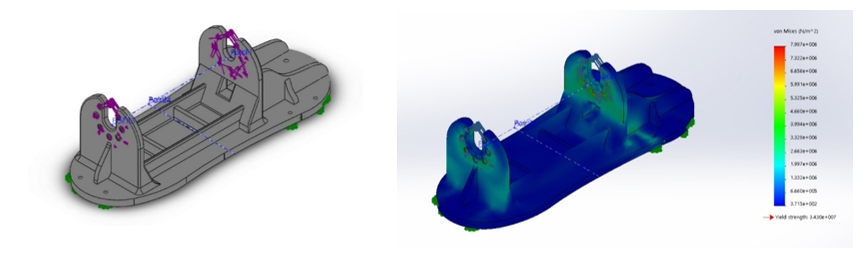
\includegraphics[width=0.9\textwidth]{chapter4/images/FEA4.PNG}
  \caption{รูปการวิเคราะห์แรงของเท้าหุ่นยนต์}
  \label{fig:FEA4}
\end{figure}

การวิเคราะห์นั้นมีวิธีการทำเหมือนกับการวิเคราะห์ชิ้นส่วนขาคือทำการยึดจุดที่เป็นหน้าแปลนของมอเตอร์ไว้เพื่อให้เปรียบเสมือนกับว่าขณะนี้ชิ้นงานได้เชื่อมติดกับตัวมอเตอร์ 
หลังจากนั้นกำหนดแรงกระทำเพื่อให้เกิดแรงบิดกับชิ้นงานโดยค่าแรงที่กระทำนั้นได้มาจากการคำณวนแรงของมอเตอร์ที่ทำกับชิ้นงานข้อเท้าที่แรงบิด 10.4 นิวตัน/เมตร $(N.m)$
ได้ผลดังตาราง \ref{tab:footstress_result}

\begin{table}[!ht]
	\centering
	\begin{tabular}{| l | c |}
		\hline
		ชื่อชิ้นงาน	& ความตึงเครียดสูงสุดของชิ้นงาน(Max stress)$(N/mm^2)$ \\
        \hline
        ฝ่าเท้า & 37.44 \\
	    \hline
	\end{tabular}
	\caption{ตารางแสดงความตึงเครียดของชิ้นงาน(Stress)ของฝ่าเท้า}
	\label{tab:footstress_result}
\end{table}

\clearpage
\subsubsection*{ปัญหาที่พบ}
เมื่อทำการประกอบชิ้นส่วนของ FSR(Force Sensitive Resistor) กับฝ่าเท้าแล้วปัญหาที่พบคือ พื้นที่สัมผัสพื้นของฝ่าเท้า
น้อยลงซึ่งเป็นผลทำให้ support polygon น้อยลงด้วยซึ่งเป็นเหตุทำให้การเดินของหุ่นยนต์นั้นยากลำบาก
\begin{figure}[h!]
  \centering
  \begin{subfigure}[b]{0.3\linewidth}
    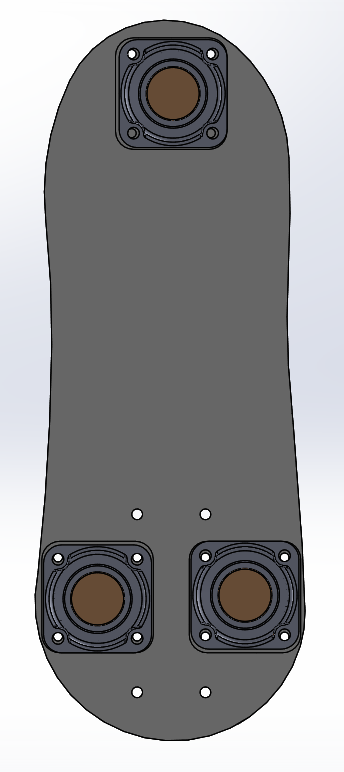
\includegraphics[width=\linewidth]{chapter4/images/foot+FSR.PNG}
    \caption{รูปแสดงเท้าของหุ่นยนต์เมื่อประกอบ FSR แล้ว}
  \end{subfigure}
  \begin{subfigure}[b]{0.3\linewidth}
    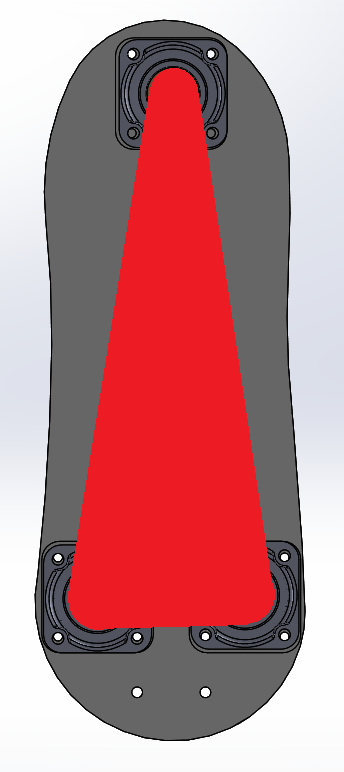
\includegraphics[width=\linewidth]{chapter4/images/foot+FSR_sp.PNG}
    \caption{รูปแสดง support polygon ของเท้าเมื่อประกอบ FSR}
  \end{subfigure}
  \caption{รูปแสดงฝ่าเท้าและ support polygon}
  \label{fig:foot_FSR}
\end{figure}

ดังนั้นจึงทำการแก้ไขโดย ออกแบบฝ่าเท้าให้มีขนาดใหญ่เพิ่มขึ้น และออกแบบเซนเซอร์ตรวจจับการเดินให้มีความบางลงอีกเพือให้หุ่นยนต์นั้น
มี support polygon เพิ่มขึ้น

\clearpage
\subsubsection{การออกแบบโครงสร้างเท้าครั้งที่ 2}
ในการออกแบบครั้งนี้ได้เพิ่มขนาดของฝ่าเท้าให้ใหญ่ขึ้นเพื่อเพิ่ม support polygon ซึ่งจะเป็นผลทำให้หุ่นยนต์นั้นมีการเดินที่ง่ายขึ้น
ในการปรับขนาดครั้งนี้ได้เพิ่มขนาดที่ปลายเท้าให้ใหญ่ขึ้น และส้นเท้ารองลงมา
\begin{figure}[!ht]
  \centering
  \begin{subfigure}[b]{0.4\linewidth}
    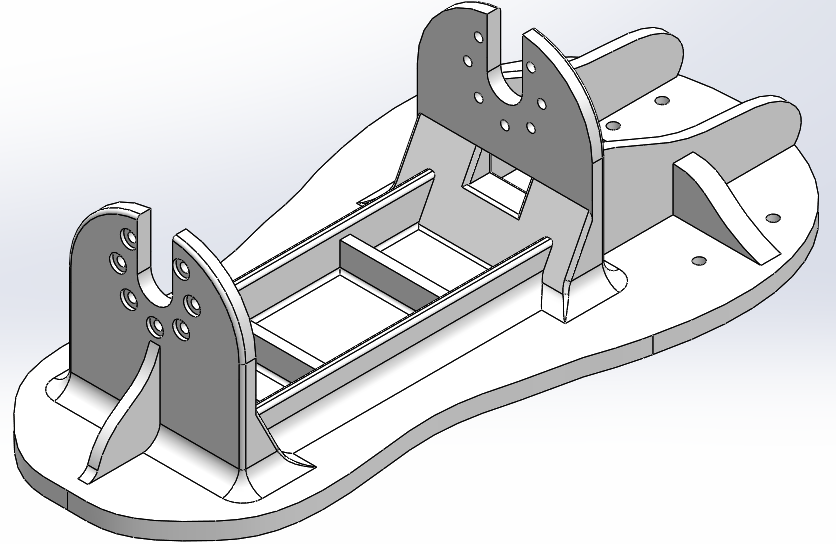
\includegraphics[width=\linewidth]{chapter4/images/foot_new.PNG}
    \caption{รูปแสดงเท้าของหุ่นยนต์ที่ออกแบบใหม่}
  \end{subfigure}
  \begin{subfigure}[b]{0.4\linewidth}
    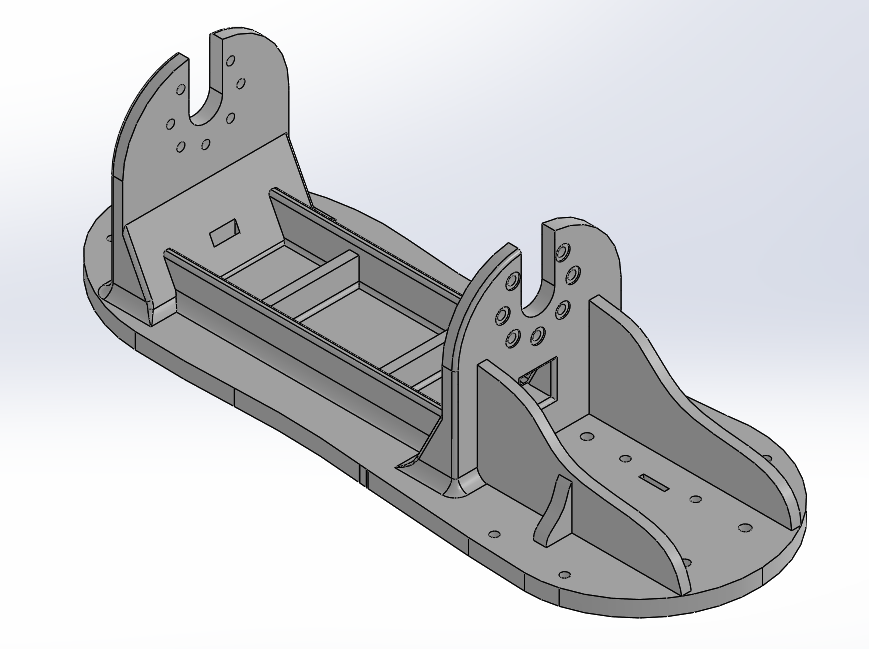
\includegraphics[width=\linewidth]{chapter4/images/foot_old.PNG}
    \caption{รูปแสดงเท้าของหุ่นยนต์เดิม}
  \end{subfigure}
  \begin{subfigure}[b]{0.2\linewidth}
    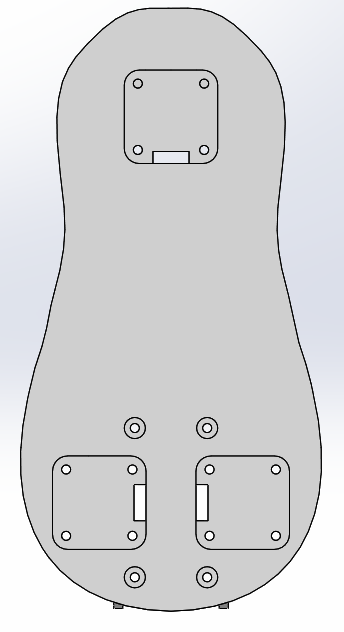
\includegraphics[width=\linewidth]{chapter4/images/bare_footnew.PNG}
    \caption{รูปแสดงฝ่าเท้าที่ออกแบบใหม่}
  \end{subfigure}
  \begin{subfigure}[b]{0.15\linewidth}
    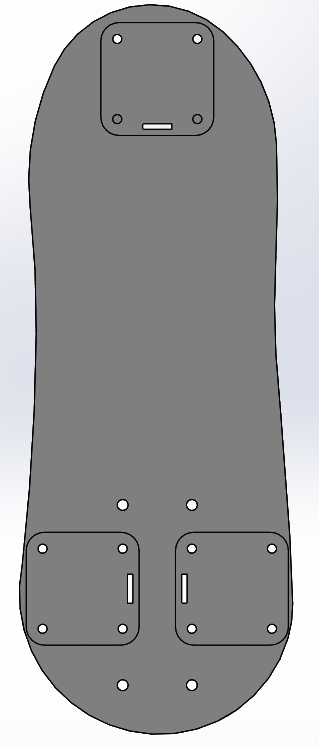
\includegraphics[width=\linewidth]{chapter4/images/bare_footold.PNG}
    \caption{รูปแสดงฝ่าเท้าเดิม}
  \end{subfigure}
  \caption{รูปแสดงการเปรียบเทียบระหว่างเท้าเดิมและเท้าที่ออกแบบใหม่}
  \label{fig:foot_compilation}
\end{figure}


ในส่วนของเซนเซอร์ตรวจจับพื้นนั้นได้ทำการออกแบบใหม่ทั้งหมดให้มีความบางลงกว่าเดิม และให้มีส่วนที่ยื่นออกมา
จากฝ่าเท้าน้อยที่สุดซึ่งความสูงที่ยื่นออกมานั้นมีสความสูงเพียง 0.4 มิลลิเมตร ต่างจากเดิมที่มีความสูงถึง 5.4 มิลลิเมตร
\begin{figure}[h!]
  \centering
  \begin{subfigure}[b]{0.3\linewidth}
    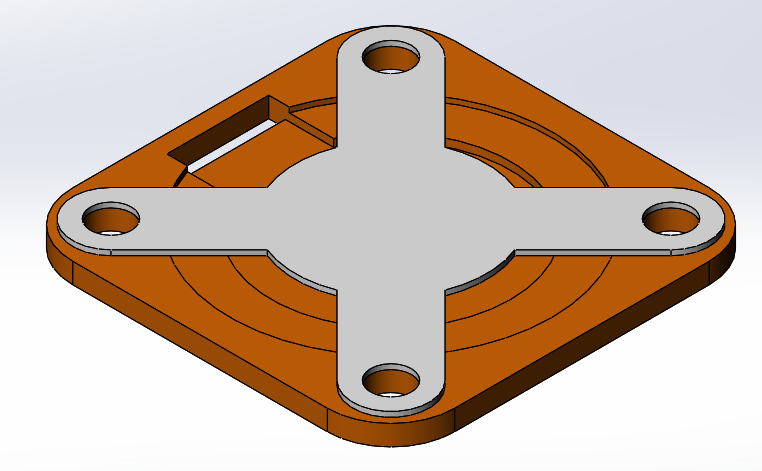
\includegraphics[width=\linewidth]{chapter4/images/FSR_new.PNG}
    \caption{รูปแสดงโครงครอบ FSR ที่ออกแบบใหม่}
  \end{subfigure}
  \begin{subfigure}[b]{0.3\linewidth}
    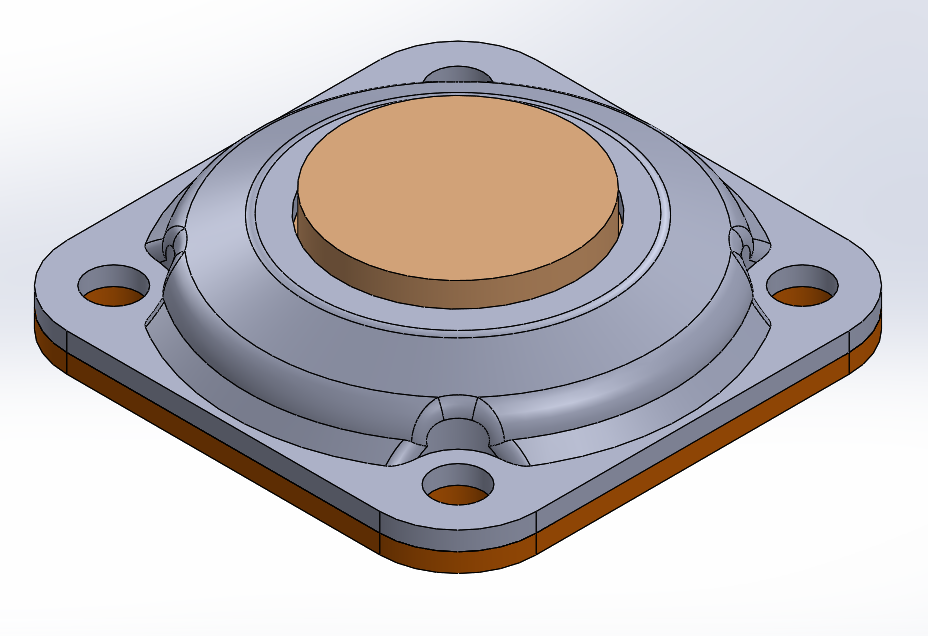
\includegraphics[width=\linewidth]{chapter4/images/FSR.PNG}
    \caption{รูปแสดงโครงครอบ FSR เดิม}
  \end{subfigure}
  \caption{รูปแสดงการเปรียบเทียบระหว่างฝ่าเท้าเดิมและฝ่าเท้าที่ออกแบบใหม่}
  \label{fig:barefoot_compilation}
\end{figure}

\subsubsection{ทดสอบการใช้งานของเซนเซอร์ตรวจจับการสัมผัสพื้น}
ในโครงงานนนี้เซนเซอร์ตรวจจับพื้นนั้นได้ใช้ใช้งานเพื่อตรวจการเหยียบของเท้าเท่านั้นว่ามีการแตะพื้นหรือไม่ ซึ่งจะกำหนดค่าไว้ในช่วง 
0-1023 โดยจะกำหนดให้ช่วงที่มากกว่า 1000 หมายถึงเท้ามีการยกเกิดขึ้นและต่ำกว่านั้นหมายถึงเท้ามีการเหยียบ โดยจะแปลงค่าเซนเซอร์ทั้ง 3 ค่าบนเท้า
เป็นค่าเฉลี่ยน้ำหนัก ตามสมการ $(sensor1 + sensor 2 + 2(sensor3))/4$ โดยให่ค่าตามแกน X เป็นค่า sampling(ครั้ง) ของข้อมูลและ
ค่าตามแกน Y เป็นค่าช่อง 0-1023 เมื่อทำการทดลองให้ทำการเหยียบเท้าและยกเท้าจะได้ผลดังภาพ \ref{fig:FSR_graph}

\begin{figure}[h!]
  \centering
  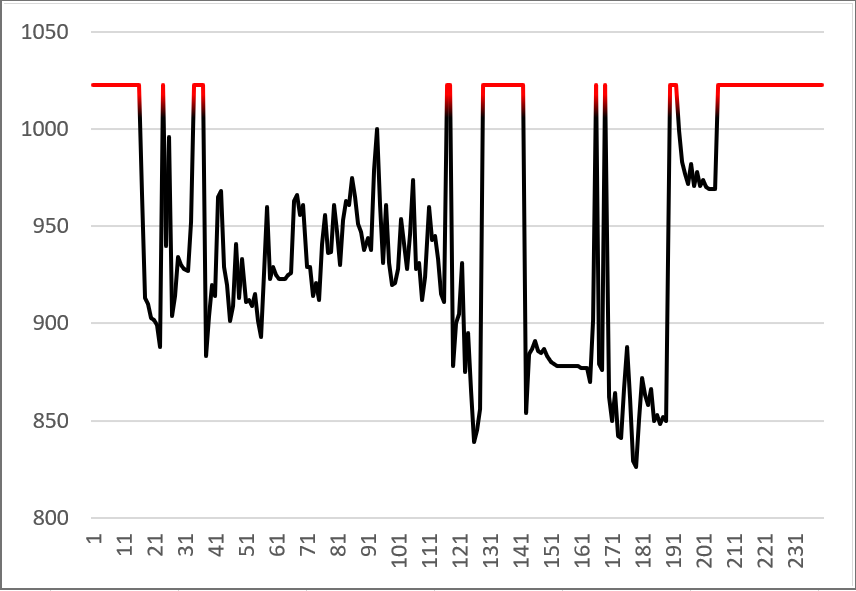
\includegraphics[width=0.6\textwidth]{chapter4/images/FSR_graph.PNG}
  \caption{รูปภาพแสดงค่าที่วัดได้ของ FSR}
  \label{fig:FSR_graph}
\end{figure}
ผลที่ได้นี้เกิดจากการทดลองยกเท้าของหุ่นยนต์ขึ้นขณะหุ่นยนต์ยืนอยู่และยกเท้าขึ้น ค่าที่อ่านได้จะมีค่า 1023 หรือสูงสุดตามภาพ และเมื่อเท้าสัมผัสพื้นนั้น
ค่าที่อ่านได้จะมีค่าที่ต่ำขึ้นอยู่กับแรงกดที่กระทำต่อเท้า ซึ่งถ้าค่าที่กระทำมากจะทำให้ค่าที่อ่านได้ต่ำมาก จะเห็นได้จากรูปภาพ \ref{fig:FSR_graph} 
จะมีช่วงเวลาหนึ่งที่ค่าที่อ่านได้ต่ำสุดซึ่งขณะนั้น ได้ทดลองกดด้วยแรงจำนวนหนึ่งที่มากกว่าน้ำหนักตัวหุ่นยนต์เป็นเวลา 1-2 วินาที


\clearpage
\subsection{การออกแบบโครงสร้างลำตัว}
ลำตัวของหุ่นยนต์นั้นจะใช้สำหรับติดตั้งหน่วยประมวลผลควบคุมระดับต่ำและระดับสูง IMU รวมไปถึงบอร์ดแปลงไฟ 12v จากแบตเตอรี่
ให้เหลือ 5V เพื่อจ่ายไฟให้กับระบบ ละยังคงต้องจัดเก็บแบตเตอรี่สำหรับทำงานไร้สายได้อีกด้วย 
\subsubsection{การออกแบบลำตัวครั้งที่ 1}
การออกแบบครั้งนี้ได้ออกแบบให้ลำตัวนั้นขึ้นรูปด้วยเครื่องพิมพ์ 3 มิติ เพื่อให้ง่ายสำหรับผู้ต่อยอดที่มีเครื่องพิมพ์เป็นของตนเอง สามารถพิมพ์
และนำมาประกอบได้ โดยส่วนของเอวนั้นจะใช้เป็นท่อคาร์บอนไฟเบอร์ขนาดเส้นผ่านศูนย์กลางขนาด 91 มิลลิเมตร เพื่อให้เหมาะสมกับชิ้นงาน
และเชื่อมยึดติดกันด้วยสกรูกับลำตัวและส่วนเอว
\begin{figure}[h!]
  \centering
  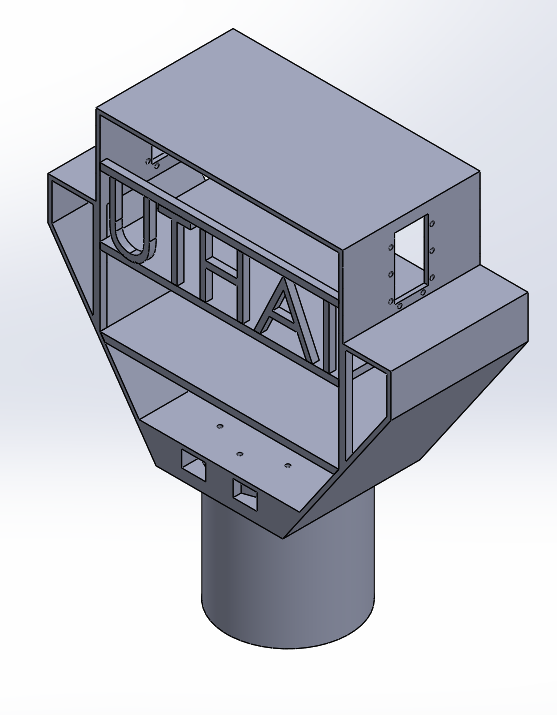
\includegraphics[width=0.4\textwidth]{chapter4/images/troso_old.PNG}
  \caption{รูปภาพแสดงตัวของหุ่นยนต์ที่ออกแบบเพื่อขึ้นรูปด้วยเครื่องพิมพ์ 3 มิติ}
  \label{fig:torso_old}
\end{figure}

แต่เมื่อทำการทดลองหาค่ามวลในโปรแกรม solidwork แล้ว ได้ผลน้ำหนักคือ 711 กรัม ซึ่งเป็นน้ำหนักที่มากเกินไปอาจส่งผลทำให้
มอเตอร์รับน้ำหนักของตัวมากเกินไป ดังนั้นจึงเป็นผลทำให้ต้องเปลี่ยนการออกแบบให้เบาลงกว่าเดิม คือลดขนาดของตัวที่ขึ้นรูปด้วยเครื่องพิมพ์ 3 มิติ
ลงและใช้วัสดุผสมระหว่างคาร์บอนไฟเบอร์มากขึ้น ซึ่งจะยังคงได้ความแข็งแรงและความเบาอีกด้วย

\clearpage
\subsubsection{การออกแบบโครงสร้างตัวครั้งที่ 2}
จากปัญหาเรื่องน้ำหนักของชิ้นส่วนตัวของการออกแบบครั้งที่ 1 ได้แก้ไขโดยลดขนาดของส่วนพิมพ์ 3 มิติลงซึ่งจะแยกชิ้นส่วนออกเป็น 2 ส่วน คือส่วนหน้าและส่วนหลัง
และใช้การยึดกับท่อคาร์บอนไฟเบอร์ซึ่งเป็นส่วนเอวด้วยการบีบซึ่งทำโดยการร้อยสกรูผ่านช่องที่ทำไว้สำเร็จบนตัวชิ้นงานพิมพ์ 3 มิติ แล้วขันให้ชิ้นงานมาประกบเข้าหากัน

\begin{figure}[h!]
  \centering
  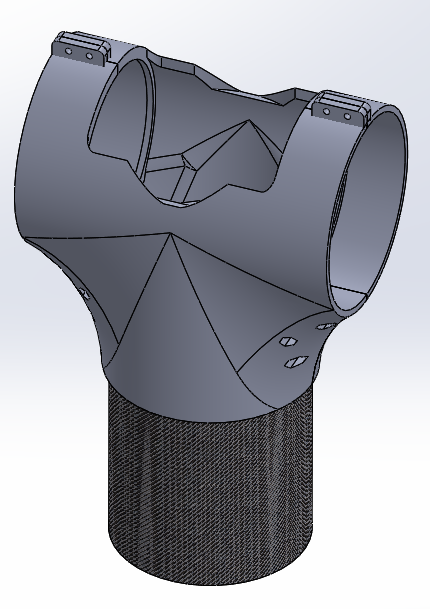
\includegraphics[width=0.4\textwidth]{chapter4/images/troso_new.PNG}
  \caption{รูปภาพแสดงตัวของหุ่นยนต์ที่ออกแบบเพื่อขึ้นรูปด้วยเครื่องพิมพ์ 3 มิติ(ใหม่)}
  \label{fig:torso_new}
\end{figure}
ซึ่งน้ำหนักที่วิเคราะห์ได้โดยโปรแกรม solidwork นั้นได้ค่าเท่ากับ 342 กรัม ซึ่งน้อยกว่าการออกแบบครั้งแรกถึง 2 เท่า ซึ่งมีน้ำหนักมากถึง 711 กรัม

\subsubsection*{การยึดลำตัวกับสะโพก}
การยึดลำตัวกับสะโพกนั้นจะใช้รูปแบบการยึดโดยการถ่างวัสดุที่ทำขึ้นมาเพื่อยึดลำตัวกับสะโพกออกผ่านสกรู 1 ตัวที่ออกแบบไว้ โดยสกรูตัวนี้จะทำหน้าที่ดึงให้ถ้วยของตัวถ่าง
เคลื่อนที่ลงมาและในขณะนั้นเองตัวถ่างด้านนอกอีก 4 ตัว จะค่อยๆขยับออกถ่างให้มีแรงบีบกับขอบท่อคาร์บอนไฟเบอร์และยึดกันอย่างแน่นตรึง

\underline{ข้อแนะนำในการยึดให้แน่นมากขึ้น}
ควรจะใช้วัสดุที่มีความหนืด เช่น ยางในรถจักรยาน หรือแผ่นกันเลื่อน ยึดกับหน้าสัมผัสของตัวถ่างก่อนแล้วจึงนำไปยึดกับวัสดุจริง)

\clearpage
\begin{figure}[h!]
  \centering
  \begin{subfigure}[b]{0.4\linewidth}
    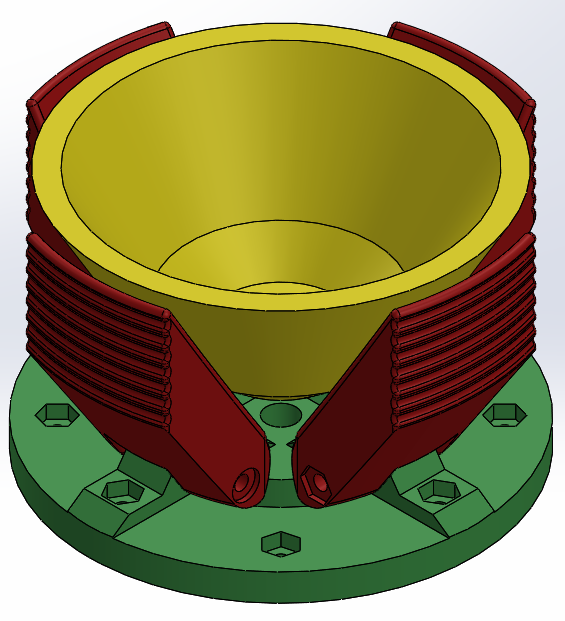
\includegraphics[width=\linewidth]{chapter4/images/hipconnector.PNG}
    \caption{รูปภาพแสดงอุปกรณ์ยึดระหว่างลำตัวกับสะโพก}
  \end{subfigure}
  \begin{subfigure}[b]{0.4\linewidth}
    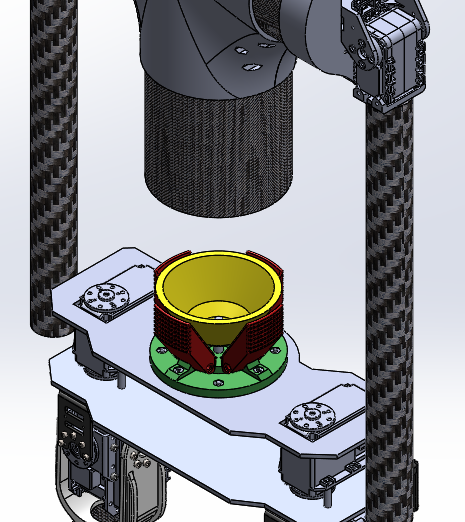
\includegraphics[width=\linewidth]{chapter4/images/explode_hipconnect.PNG}
    \caption{รูปภาพแสดงการติดตั้งบนสะโพกพร้อมทำการยึดกับลำตัวหุ่นยนต์}
  \end{subfigure}
  \caption{รูปแสดงการใช้งานส่วนยึดสะโพกกับลำตัว}
  \label{fig:barefoot_compilation}
\end{figure}

\subsubsection*{การติดตั้งบอร์ดควบคุมและแบตเตอรี่}
เนื่องจากว่าบอร์ดควบคุมทั้ง 2 (Nucleo f411re,Odroid XU4)นั้นมีขนาดที่กระทัดรัด รวมถึงบอร์ด IMU และบอร์ดแปลงไฟ ที่มีขนาดเล็กเช่นกัน ฉะนั้นจึงได้ออกแบบ
ฐานสำหรับยึดบอร์ดทั้งหมดไว้ในที่เดียว และเมื่อติดตั้งในฐานเรียบร้อยแล้วก็สามารถนำฐานนั้น สวมลงไปในตัวของหุ่นยนต์ได้พอดี
\begin{figure}[h!]
  \centering
  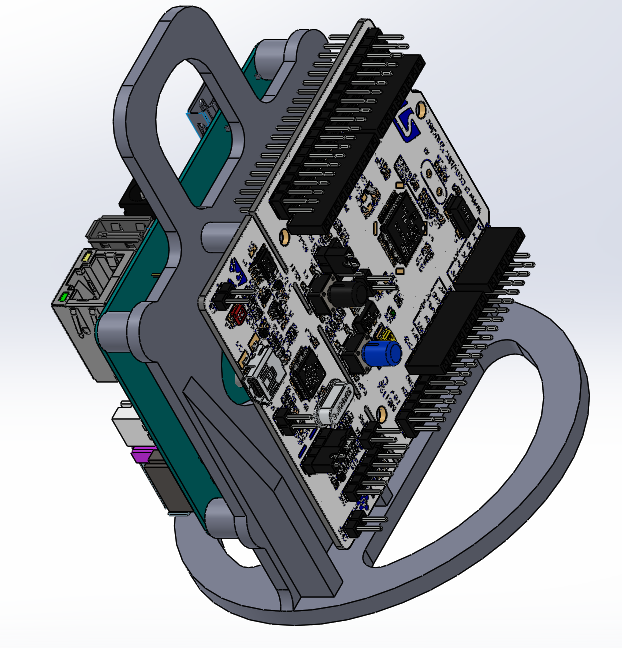
\includegraphics[width=0.4\textwidth]{chapter4/images/board_hold.PNG}
  \caption{รูปภาพแสดงฐานที่ติดตั้งบอร์ดควบคุม}
  \label{fig:board_hold}
\end{figure}
 
\clearpage
\begin{figure}[h!]
  \centering
  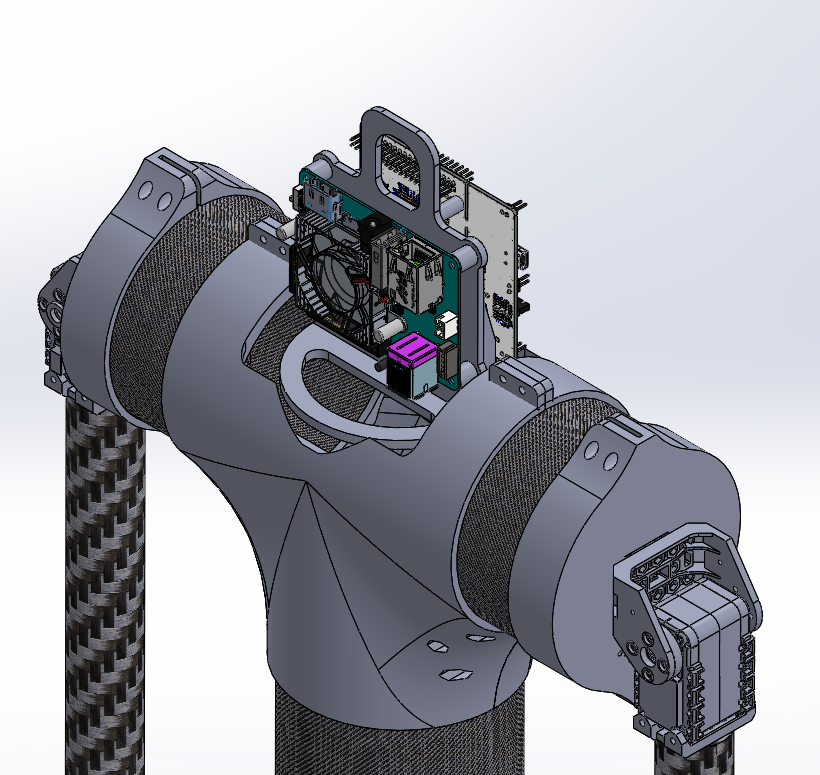
\includegraphics[width=0.4\textwidth]{chapter4/images/install_board.PNG}
  \caption{รูปภาพแสดงตฐานที่ติดตั้งบอร์ดควบคุมในตัวของหุ่นยนต์}
  \label{fig:install_board}
\end{figure}

ซึ่งเมื่อทำการติดตั้งในตัวหุ่นยนต์แล้ว การยึดติดกับบอร์ดนั้นใช้หลักการยึดเดียวกับการยืดท่อคาร์บอนกับลำตัวคือ
ใช้แรงของการบีบอัดจากสกรูบนลำตัวทั้งหมด ยึดให้อยู่กับที่ ส่วนของแบตเตอรี่นั้นจะใช้เป็นแบตเตอรี่ขนาด 6000$mAh$ 12.6V
จะถูกติดตั้งในส่วนลำตัวของหุ่นยนต์บริเวณท่อคาร์บอนไฟเบอร์

\subsubsection{การออกแบบแขน}
แขนนั้นได้ออกแบบให้เรียบง่ายและน้ำหนักเบา ซึ่งในโครงงานนี้แขนจะเป็นหนึ่งในตัวแปรที่ช่วยในการเดินให้คล่องแคล่วมากขึ้น
โดยวัสดุหลักที่ใช้มาทำแขนนั้นจะมาจากวัสดุคาร์บอนไฟเบอร์เป็นหลักและชิ้นส่วนพิมพ์ 3 มิติจะใช้สำหรับเชื่อมวัสดุทั้งหมดเข้าด้วยกัน
\begin{figure}[h!]
  \centering
  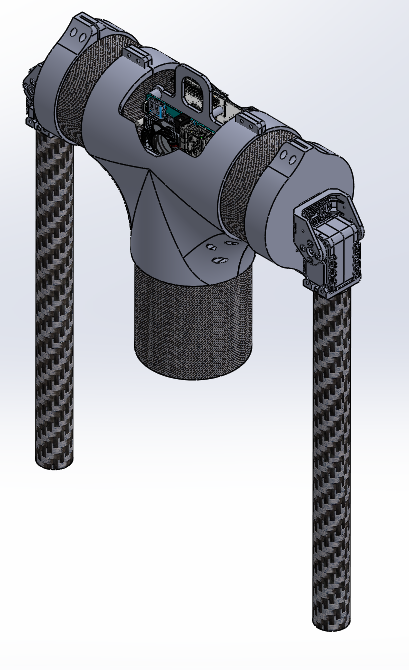
\includegraphics[width=0.4\textwidth]{chapter4/images/troso.PNG}
  \caption{รูปภาพแสดงตัวของหุ่นยนต์ที่ติดตั้งแขนทั้ง 2 ข้าง}
  \label{fig:troso}
\end{figure}

% \subsection{น้ำหนักตัวหุ่นยนต์}
% หลังจากออกแบบและจัดทำชิ้นส่วนทั้งหมดเสร็จสมบูรณ์ ได้ทำการชั่งน้ำหนักของชิ้นส่วนทั้งหมดเพื่อหาน้ำหนักจริง
% เปรียบเทียบกับค่าที่ได้จากโปรแกรม solidwork ซึ่งผลที่ได้นี้จะเป็นน้ำหนักที่ยังไม่รวมน้ำหนักมอเตอร์ ทั้ง 14 ตัว
% และแบตเตอรี่ จะได้ผลดังตาราง
% \begin{table}[ht]
% 	\centering
% 	\begin{tabular}{| l | c | c |}
% 		\hline
% 		ชื่อชิ้นงาน	& น้ำหนักที่ชั่งจริง (กรัม) & น้ำหนักในโปรแกรม 3 มิติ (กรัม) \\
%         \hline
%         ลำตัว & & 342 \\
%         แขนซ้าย  & 272 & 241\\
%         แขนขวา  & 272 & 241\\
%         ต้นขา & 154 & 161 \\
%         หน้าแข้ง & 138 & \\
%         เท้า & & 148\\
% 	    \hline
% 	\end{tabular}
% 	\caption{ตารางแสดงความตึงเครียดของชิ้นงาน(Stress)}
% 	\label{tab:stress_result}
% \end{table}


\clearpage
\subsection{Engineer drawing}

\begin{figure}[!ht]
  \centering
  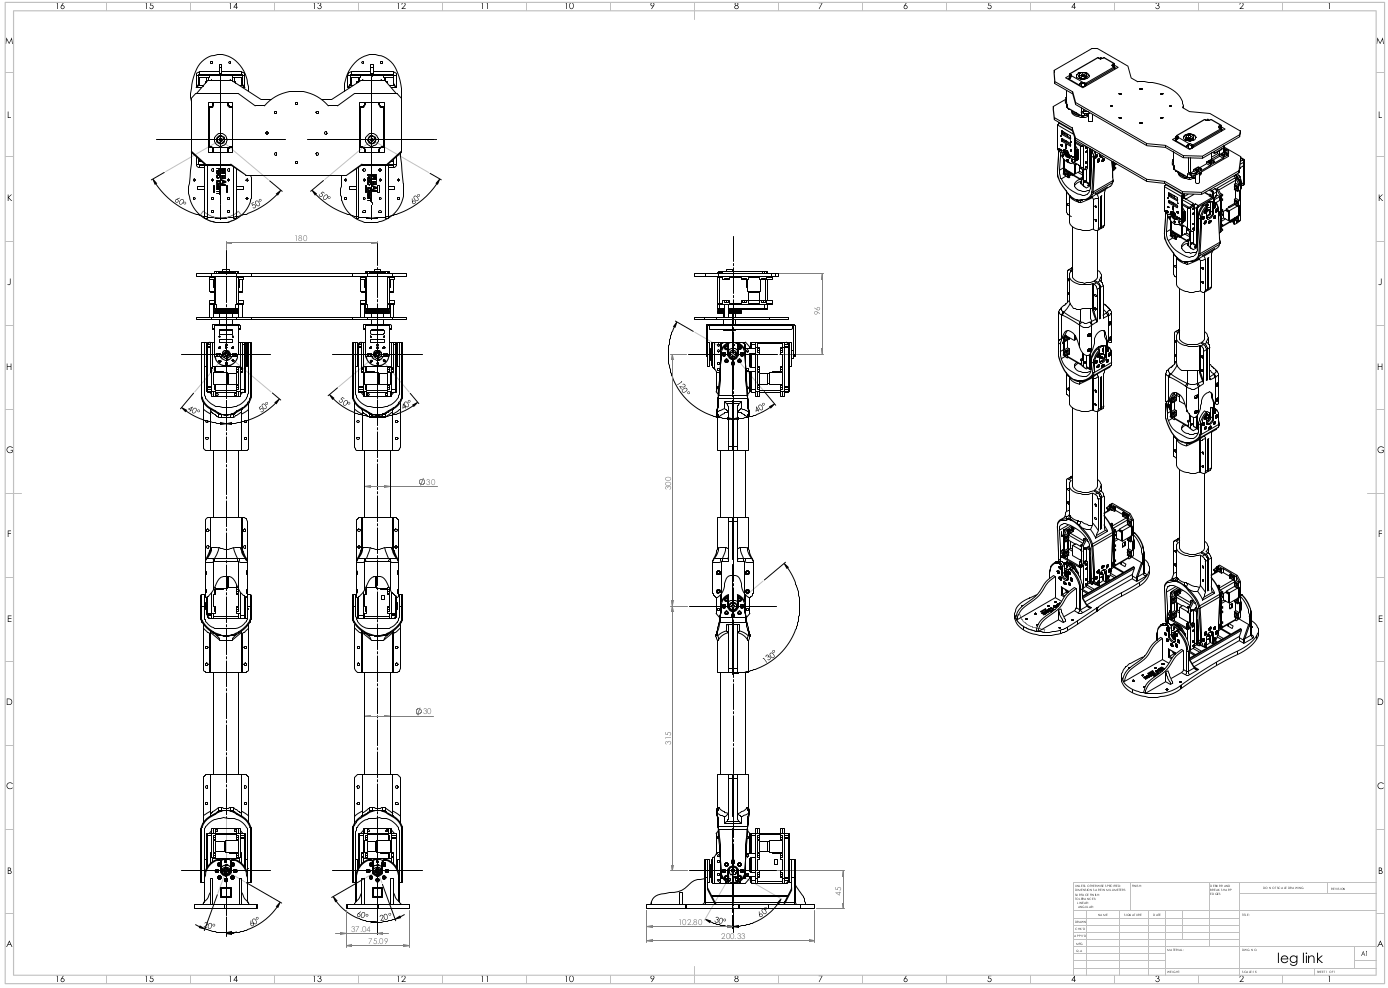
\includegraphics[width=0.8\textwidth]{chapter4/images/uthai_drawing_leg.png}
  \caption{ภาพ drawing ของขาหุ่นยนต์ฮิวมานอยด์อุทัย}
  \label{fig:uthai_drawing_leg}
\end{figure}
\begin{figure}[!ht]
  \centering
  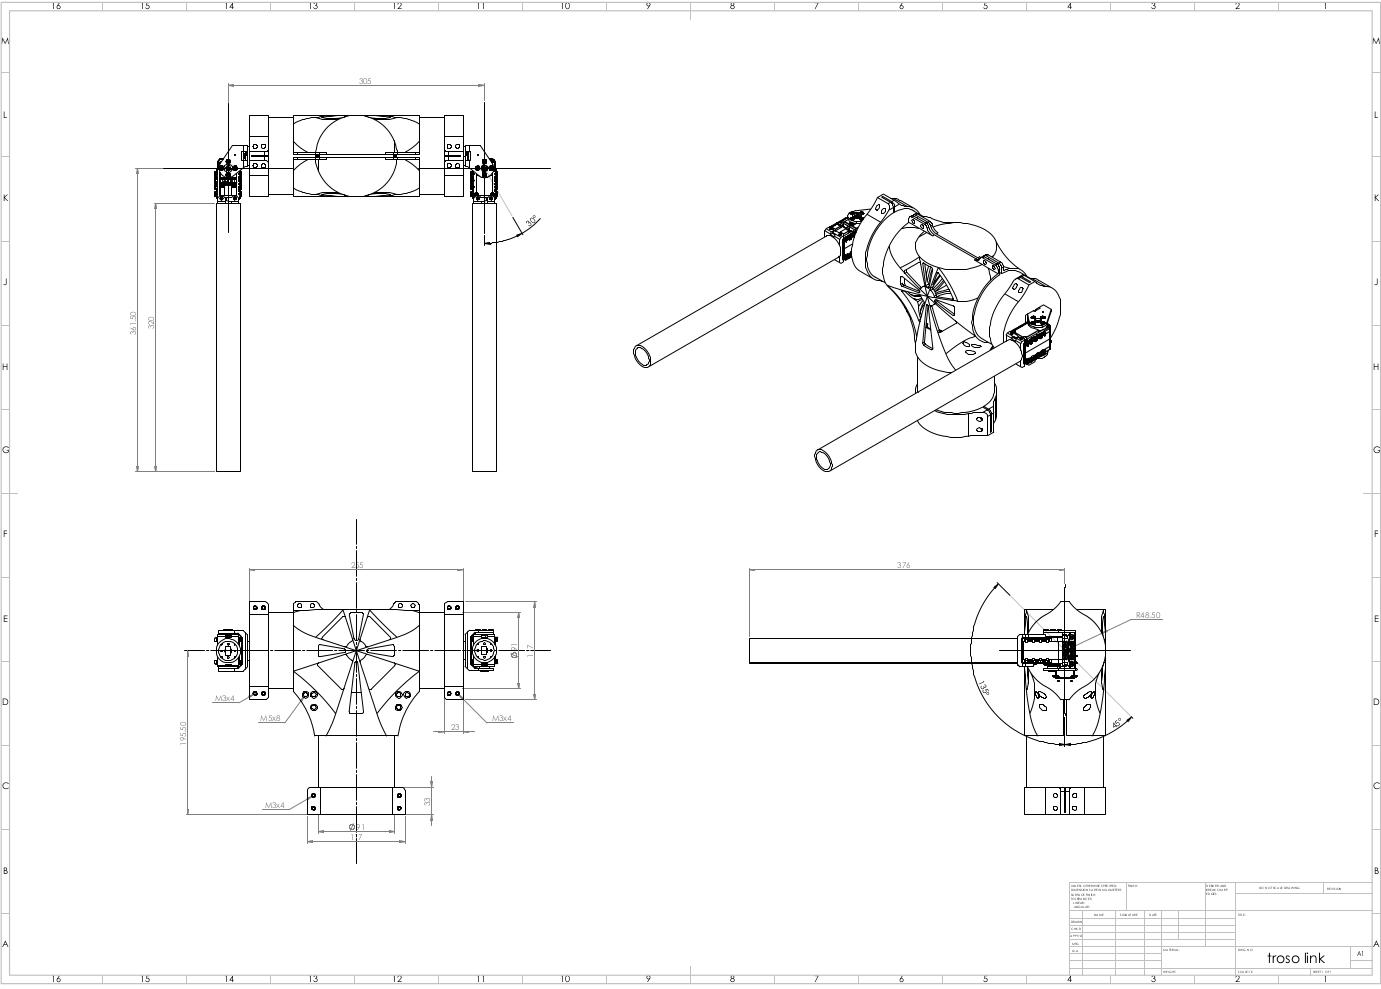
\includegraphics[width=0.8\textwidth]{chapter4/images/uthai_drawing_body.png}
  \caption{ภาพ drawing ของตัวหุ่นยนต์ฮิวมานอยด์อุทัย}
  \label{fig:uthai_drawing_body}
\end{figure}